\documentclass{standalone}
\usepackage{tikz}
\usetikzlibrary{patterns, positioning}
\usepackage[sfdefault]{ClearSans} %% option 'sfdefault' activates Clear Sans as the default text font
\usepackage[T1]{fontenc}

\begin{document}
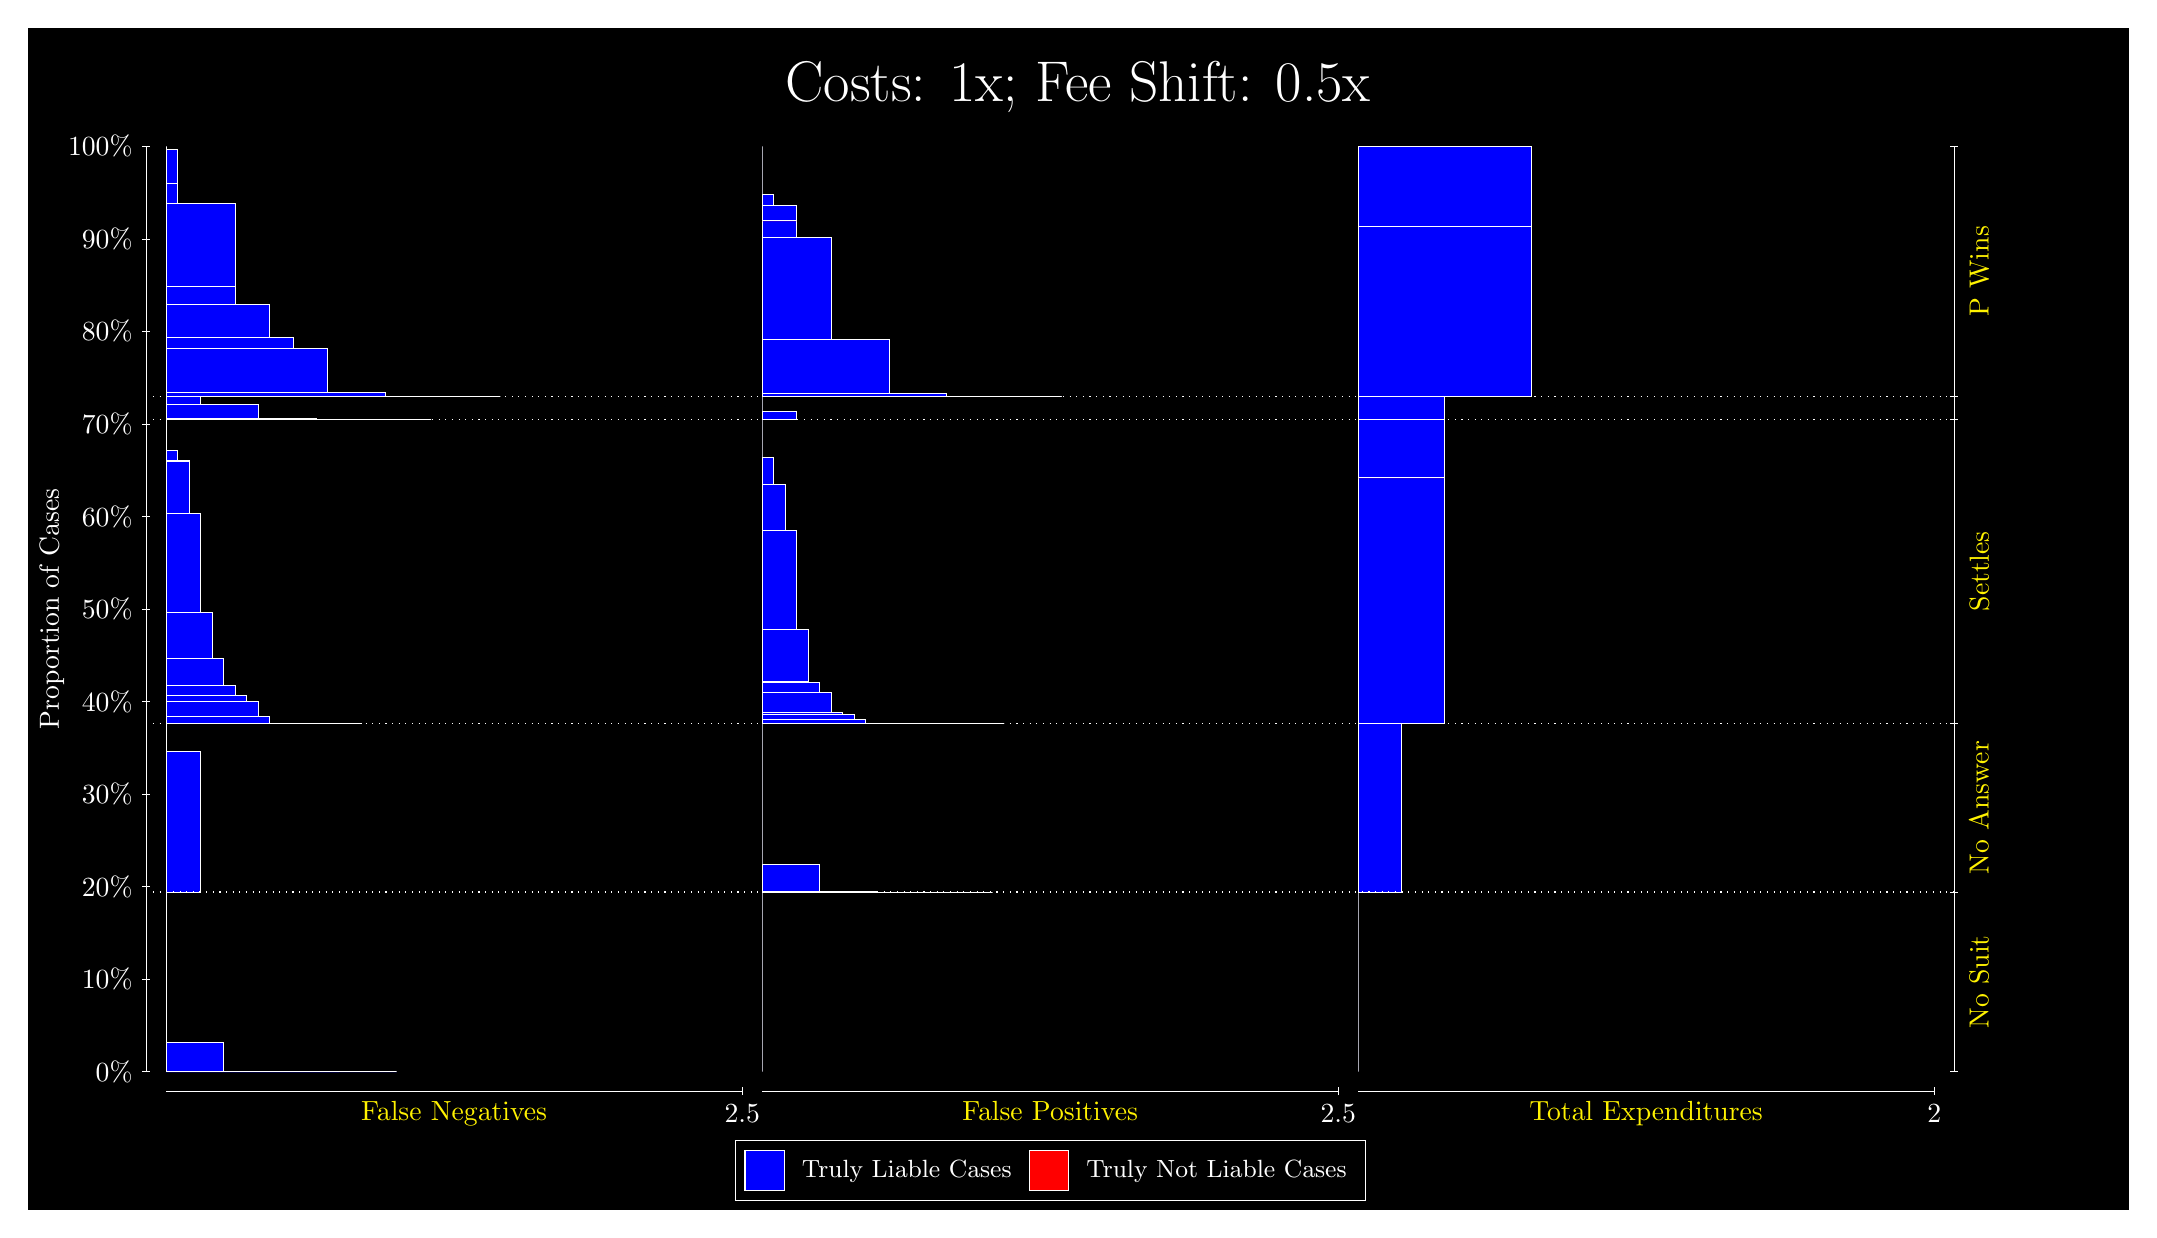
\begin{tikzpicture}
\draw[fill=black] (0,0) rectangle (26.667,15);
\draw[text=white] (0,13.5) rectangle (26.667,15) node[midway] {\huge Costs: 1x; Fee Shift: 0.5x};
\draw[white, very thin] (1.5,1.75) -- (1.5,13.5);
\node[rotate=90, text=white, anchor=center] at (0.3, 7.625) {Proportion of Cases};
\draw[white, very thin] (1.45,1.75) -- (1.55,1.75);
\node[text=white, anchor=east] at (1.45, 1.75) {0\%};
\draw[white, very thin] (1.45,2.925) -- (1.55,2.925);
\node[text=white, anchor=east] at (1.45, 2.925) {10\%};
\draw[white, very thin] (1.45,4.1) -- (1.55,4.1);
\node[text=white, anchor=east] at (1.45, 4.1) {20\%};
\draw[white, very thin] (1.45,5.275) -- (1.55,5.275);
\node[text=white, anchor=east] at (1.45, 5.275) {30\%};
\draw[white, very thin] (1.45,6.45) -- (1.55,6.45);
\node[text=white, anchor=east] at (1.45, 6.45) {40\%};
\draw[white, very thin] (1.45,7.625) -- (1.55,7.625);
\node[text=white, anchor=east] at (1.45, 7.625) {50\%};
\draw[white, very thin] (1.45,8.8) -- (1.55,8.8);
\node[text=white, anchor=east] at (1.45, 8.8) {60\%};
\draw[white, very thin] (1.45,9.975) -- (1.55,9.975);
\node[text=white, anchor=east] at (1.45, 9.975) {70\%};
\draw[white, very thin] (1.45,11.15) -- (1.55,11.15);
\node[text=white, anchor=east] at (1.45, 11.15) {80\%};
\draw[white, very thin] (1.45,12.325) -- (1.55,12.325);
\node[text=white, anchor=east] at (1.45, 12.325) {90\%};
\draw[white, very thin] (1.45,13.5) -- (1.55,13.5);
\node[text=white, anchor=east] at (1.45, 13.5) {100\%};

\draw[white, very thin] (24.457,1.75) -- (24.457,13.5);
\draw[white, very thin] (24.407,1.75) -- (24.507,1.75);
\node[anchor=west] at (24.407, 1.75) {};
\draw[white, very thin] (24.407,4.0302) -- (24.507,4.0302);
\node[anchor=west] at (24.407, 4.0302) {};
\draw[white, very thin] (24.407,6.1731) -- (24.507,6.1731);
\node[anchor=west] at (24.407, 6.1731) {};
\draw[white, very thin] (24.407,10.036) -- (24.507,10.036);
\node[anchor=west] at (24.407, 10.036) {};
\draw[white, very thin] (24.407,10.326) -- (24.507,10.326);
\node[anchor=west] at (24.407, 10.326) {};
\draw[white, very thin] (24.407,13.5) -- (24.507,13.5);
\node[anchor=west] at (24.407, 13.5) {};

\draw[white, very thin, fill=blue] (1.75,1.75) rectangle (4.6775,1.75);
\draw[white, very thin, fill=blue] (1.75,1.75) rectangle (3.9457,1.75);
\draw[white, very thin, fill=blue] (1.75,1.75) rectangle (3.2138,1.7532);
\draw[white, very thin, fill=blue] (1.75,1.7532) rectangle (2.4819,2.1234);
\draw[white, very thin, fill=red] (1.75,2.1234) rectangle (1.75,2.1234);
\draw[white, very thin, fill=blue] (1.75,2.1234) rectangle (1.75,4.0302);
\draw[white, very thin, fill=blue] (1.75,4.0302) rectangle (2.1891,5.8222);
\draw[white, very thin, fill=red] (1.75,5.8222) rectangle (1.75,5.8222);
\draw[white, very thin, fill=blue] (1.75,5.8222) rectangle (1.75,6.1731);
\draw[white, very thin, fill=blue] (1.75,6.1731) rectangle (4.2384,6.1731);
\draw[white, very thin, fill=blue] (1.75,6.1731) rectangle (3.9457,6.1731);
\draw[white, very thin, fill=blue] (1.75,6.1731) rectangle (3.6529,6.1734);
\draw[white, very thin, fill=blue] (1.75,6.1734) rectangle (3.5065,6.1734);
\draw[white, very thin, fill=blue] (1.75,6.1734) rectangle (3.3602,6.1738);
\draw[white, very thin, fill=blue] (1.75,6.1738) rectangle (3.2138,6.1754);
\draw[white, very thin, fill=blue] (1.75,6.1754) rectangle (3.0674,6.261);
\draw[white, very thin, fill=blue] (1.75,6.261) rectangle (2.921,6.4469);
\draw[white, very thin, fill=blue] (1.75,6.4469) rectangle (2.7746,6.5265);
\draw[white, very thin, fill=blue] (1.75,6.5265) rectangle (2.6283,6.653);
\draw[white, very thin, fill=blue] (1.75,6.653) rectangle (2.4819,7.0045);
\draw[white, very thin, fill=blue] (1.75,7.0045) rectangle (2.3355,7.5886);
\draw[white, very thin, fill=blue] (1.75,7.5886) rectangle (2.1891,8.8391);
\draw[white, very thin, fill=blue] (1.75,8.8391) rectangle (2.0428,9.4981);
\draw[white, very thin, fill=blue] (1.75,9.4981) rectangle (2.0428,9.5142);
\draw[white, very thin, fill=blue] (1.75,9.5142) rectangle (1.8964,9.6404);
\draw[white, very thin, fill=red] (1.75,9.6404) rectangle (1.75,9.6404);
\draw[white, very thin, fill=blue] (1.75,9.6404) rectangle (1.75,10.036);
\draw[white, very thin, fill=blue] (1.75,10.036) rectangle (5.1167,10.036);
\draw[white, very thin, fill=blue] (1.75,10.036) rectangle (4.3848,10.036);
\draw[white, very thin, fill=blue] (1.75,10.036) rectangle (3.6529,10.043);
\draw[white, very thin, fill=blue] (1.75,10.043) rectangle (2.921,10.224);
\draw[white, very thin, fill=blue] (1.75,10.224) rectangle (2.1891,10.326);
\draw[white, very thin, fill=red] (1.75,10.326) rectangle (1.75,10.326);
\draw[white, very thin, fill=blue] (1.75,10.326) rectangle (5.9949,10.326);
\draw[white, very thin, fill=blue] (1.75,10.326) rectangle (5.2631,10.327);
\draw[white, very thin, fill=blue] (1.75,10.327) rectangle (4.8239,10.327);
\draw[white, very thin, fill=blue] (1.75,10.327) rectangle (4.5312,10.376);
\draw[white, very thin, fill=blue] (1.75,10.376) rectangle (4.092,10.376);
\draw[white, very thin, fill=blue] (1.75,10.376) rectangle (3.7993,10.933);
\draw[white, very thin, fill=blue] (1.75,10.933) rectangle (3.3602,11.077);
\draw[white, very thin, fill=blue] (1.75,11.077) rectangle (3.0674,11.488);
\draw[white, very thin, fill=blue] (1.75,11.488) rectangle (2.6283,11.724);
\draw[white, very thin, fill=blue] (1.75,11.724) rectangle (2.6283,12.778);
\draw[white, very thin, fill=blue] (1.75,12.778) rectangle (2.3355,12.778);
\draw[white, very thin, fill=blue] (1.75,12.778) rectangle (1.8964,13.034);
\draw[white, very thin, fill=blue] (1.75,13.034) rectangle (1.8964,13.458);
\draw[white, very thin, fill=red] (1.75,13.458) rectangle (1.75,13.458);
\draw[white, very thin, fill=blue] (1.75,13.458) rectangle (1.75,13.5);
\draw[white, very thin, fill=red] (9.3189,1.75) rectangle (9.3189,1.75);
\draw[white, very thin, fill=blue] (9.3189,1.75) rectangle (9.3189,4.0302);
\draw[white, very thin, fill=red] (9.3189,4.0302) rectangle (12.246,4.0302);
\draw[white, very thin, fill=blue] (9.3189,4.0302) rectangle (12.246,4.0302);
\draw[white, very thin, fill=blue] (9.3189,4.0302) rectangle (11.515,4.0302);
\draw[white, very thin, fill=blue] (9.3189,4.0302) rectangle (10.783,4.0332);
\draw[white, very thin, fill=blue] (9.3189,4.0332) rectangle (10.051,4.3811);
\draw[white, very thin, fill=blue] (9.3189,4.3811) rectangle (9.3189,6.1731);
\draw[white, very thin, fill=red] (9.3189,6.1731) rectangle (12.393,6.1731);
\draw[white, very thin, fill=blue] (9.3189,6.1731) rectangle (12.393,6.1731);
\draw[white, very thin, fill=red] (9.3189,6.1731) rectangle (12.1,6.1731);
\draw[white, very thin, fill=blue] (9.3189,6.1731) rectangle (12.1,6.1731);
\draw[white, very thin, fill=red] (9.3189,6.1731) rectangle (11.807,6.1731);
\draw[white, very thin, fill=blue] (9.3189,6.1731) rectangle (11.807,6.1731);
\draw[white, very thin, fill=blue] (9.3189,6.1731) rectangle (11.661,6.1731);
\draw[white, very thin, fill=red] (9.3189,6.1731) rectangle (11.515,6.1731);
\draw[white, very thin, fill=blue] (9.3189,6.1731) rectangle (11.515,6.1731);
\draw[white, very thin, fill=blue] (9.3189,6.1731) rectangle (11.368,6.1731);
\draw[white, very thin, fill=red] (9.3189,6.1731) rectangle (11.222,6.1731);
\draw[white, very thin, fill=blue] (9.3189,6.1731) rectangle (11.222,6.1731);
\draw[white, very thin, fill=blue] (9.3189,6.1731) rectangle (11.075,6.1731);
\draw[white, very thin, fill=red] (9.3189,6.1731) rectangle (10.929,6.1731);
\draw[white, very thin, fill=blue] (9.3189,6.1731) rectangle (10.929,6.1738);
\draw[white, very thin, fill=blue] (9.3189,6.1738) rectangle (10.783,6.174);
\draw[white, very thin, fill=blue] (9.3189,6.174) rectangle (10.636,6.1741);
\draw[white, very thin, fill=red] (9.3189,6.1741) rectangle (10.636,6.1741);
\draw[white, very thin, fill=blue] (9.3189,6.1741) rectangle (10.636,6.2234);
\draw[white, very thin, fill=blue] (9.3189,6.2234) rectangle (10.49,6.283);
\draw[white, very thin, fill=blue] (9.3189,6.283) rectangle (10.344,6.3123);
\draw[white, very thin, fill=blue] (9.3189,6.3123) rectangle (10.197,6.569);
\draw[white, very thin, fill=blue] (9.3189,6.569) rectangle (10.051,6.6953);
\draw[white, very thin, fill=blue] (9.3189,6.6953) rectangle (9.9044,6.7114);
\draw[white, very thin, fill=blue] (9.3189,6.7114) rectangle (9.9044,7.3704);
\draw[white, very thin, fill=blue] (9.3189,7.3704) rectangle (9.758,8.6209);
\draw[white, very thin, fill=blue] (9.3189,8.6209) rectangle (9.6116,9.205);
\draw[white, very thin, fill=blue] (9.3189,9.205) rectangle (9.4652,9.5564);
\draw[white, very thin, fill=blue] (9.3189,9.5564) rectangle (9.3189,10.036);
\draw[white, very thin, fill=red] (9.3189,10.036) rectangle (9.758,10.036);
\draw[white, very thin, fill=blue] (9.3189,10.036) rectangle (9.758,10.139);
\draw[white, very thin, fill=blue] (9.3189,10.139) rectangle (9.3189,10.326);
\draw[white, very thin, fill=red] (9.3189,10.326) rectangle (13.125,10.326);
\draw[white, very thin, fill=blue] (9.3189,10.326) rectangle (13.125,10.326);
\draw[white, very thin, fill=red] (9.3189,10.326) rectangle (12.393,10.326);
\draw[white, very thin, fill=blue] (9.3189,10.326) rectangle (12.393,10.327);
\draw[white, very thin, fill=red] (9.3189,10.327) rectangle (11.661,10.327);
\draw[white, very thin, fill=blue] (9.3189,10.327) rectangle (11.661,10.368);
\draw[white, very thin, fill=red] (9.3189,10.368) rectangle (11.222,10.368);
\draw[white, very thin, fill=blue] (9.3189,10.368) rectangle (11.222,10.368);
\draw[white, very thin, fill=red] (9.3189,10.368) rectangle (10.929,10.368);
\draw[white, very thin, fill=blue] (9.3189,10.368) rectangle (10.929,11.048);
\draw[white, very thin, fill=red] (9.3189,11.048) rectangle (10.49,11.048);
\draw[white, very thin, fill=blue] (9.3189,11.048) rectangle (10.49,11.048);
\draw[white, very thin, fill=blue] (9.3189,11.048) rectangle (10.197,12.339);
\draw[white, very thin, fill=blue] (9.3189,12.339) rectangle (9.758,12.557);
\draw[white, very thin, fill=red] (9.3189,12.557) rectangle (9.758,12.557);
\draw[white, very thin, fill=blue] (9.3189,12.557) rectangle (9.758,12.75);
\draw[white, very thin, fill=blue] (9.3189,12.75) rectangle (9.4652,12.894);
\draw[white, very thin, fill=blue] (9.3189,12.894) rectangle (9.3189,13.5);
\draw[white, very thin, fill=red] (16.888,1.75) rectangle (16.888,1.75);
\draw[white, very thin, fill=blue] (16.888,1.75) rectangle (16.888,4.0302);
\draw[white, very thin, fill=red] (16.888,4.0302) rectangle (17.437,4.0302);
\draw[white, very thin, fill=blue] (16.888,4.0302) rectangle (17.437,6.1731);
\draw[white, very thin, fill=red] (16.888,6.1731) rectangle (17.986,6.1731);
\draw[white, very thin, fill=blue] (16.888,6.1731) rectangle (17.986,9.2932);
\draw[white, very thin, fill=red] (16.888,9.2932) rectangle (17.986,9.2932);
\draw[white, very thin, fill=blue] (16.888,9.2932) rectangle (17.986,10.036);
\draw[white, very thin, fill=red] (16.888,10.036) rectangle (17.986,10.036);
\draw[white, very thin, fill=blue] (16.888,10.036) rectangle (17.986,10.326);
\draw[white, very thin, fill=red] (16.888,10.326) rectangle (19.083,10.326);
\draw[white, very thin, fill=blue] (16.888,10.326) rectangle (19.083,12.482);
\draw[white, very thin, fill=red] (16.888,12.482) rectangle (19.083,12.482);
\draw[white, very thin, fill=blue] (16.888,12.482) rectangle (19.083,13.5);
\draw[white, dotted] (1.5,4.0302) -- (24.457,4.0302);
\draw[white, dotted] (1.5,6.1731) -- (24.457,6.1731);
\draw[white, dotted] (1.5,10.036) -- (24.457,10.036);
\draw[white, dotted] (1.5,10.326) -- (24.457,10.326);
\draw[white, very thin] (1.75,1.5) -- (9.0689,1.5);
\node[text=yellow, anchor=north] at (5.4094, 1.5) {False Negatives};
\draw[white, very thin] (9.0689,1.45) -- (9.0689,1.55);
\node[text=white, anchor=north] at (9.0689, 1.45) {2.5};

\draw[white, very thin] (9.3189,1.5) -- (16.638,1.5);
\node[text=yellow, anchor=north] at (12.978, 1.5) {False Positives};
\draw[white, very thin] (16.638,1.45) -- (16.638,1.55);
\node[text=white, anchor=north] at (16.638, 1.45) {2.5};

\draw[white, very thin] (16.888,1.5) -- (24.207,1.5);
\node[text=yellow, anchor=north] at (20.547, 1.5) {Total Expenditures};
\draw[white, very thin] (24.207,1.45) -- (24.207,1.55);
\node[text=white, anchor=north] at (24.207, 1.45) {2};

\node[text=yellow, centered, rotate=90] at (24.777, 2.8901) {No Suit};
\node[text=yellow, centered, rotate=90] at (24.777, 5.1016) {No Answer};
\node[text=yellow, centered, rotate=90] at (24.777, 8.1047) {Settles};

\node[text=yellow, centered, rotate=90] at (24.777, 11.913) {P Wins};

\draw (12.978300999999998,1.5) node[draw=none] (baseCoordinate) {};
\begin{scope}[align=center]
        \matrix[scale=0.5, draw=white, below=0.5cm of baseCoordinate, nodes={draw}, column sep=0.1cm]{
            \node[rectangle, draw, minimum width=0.5cm, minimum height=0.5cm, fill=blue] {}; &
            \node[draw=none, font=\small, text=white] (B) {Truly Liable Cases}; &
            \node[rectangle, draw, minimum width=0.5cm, minimum height=0.5cm, fill=red] {}; &
            \node[draw=none, font=\small, text=white] (B) {Truly Not Liable Cases}; \\
            };
\end{scope}

\end{tikzpicture}
\end{document}